\documentclass{standalone}
\usepackage{tikz}
\usetikzlibrary{patterns, positioning}

\begin{document}
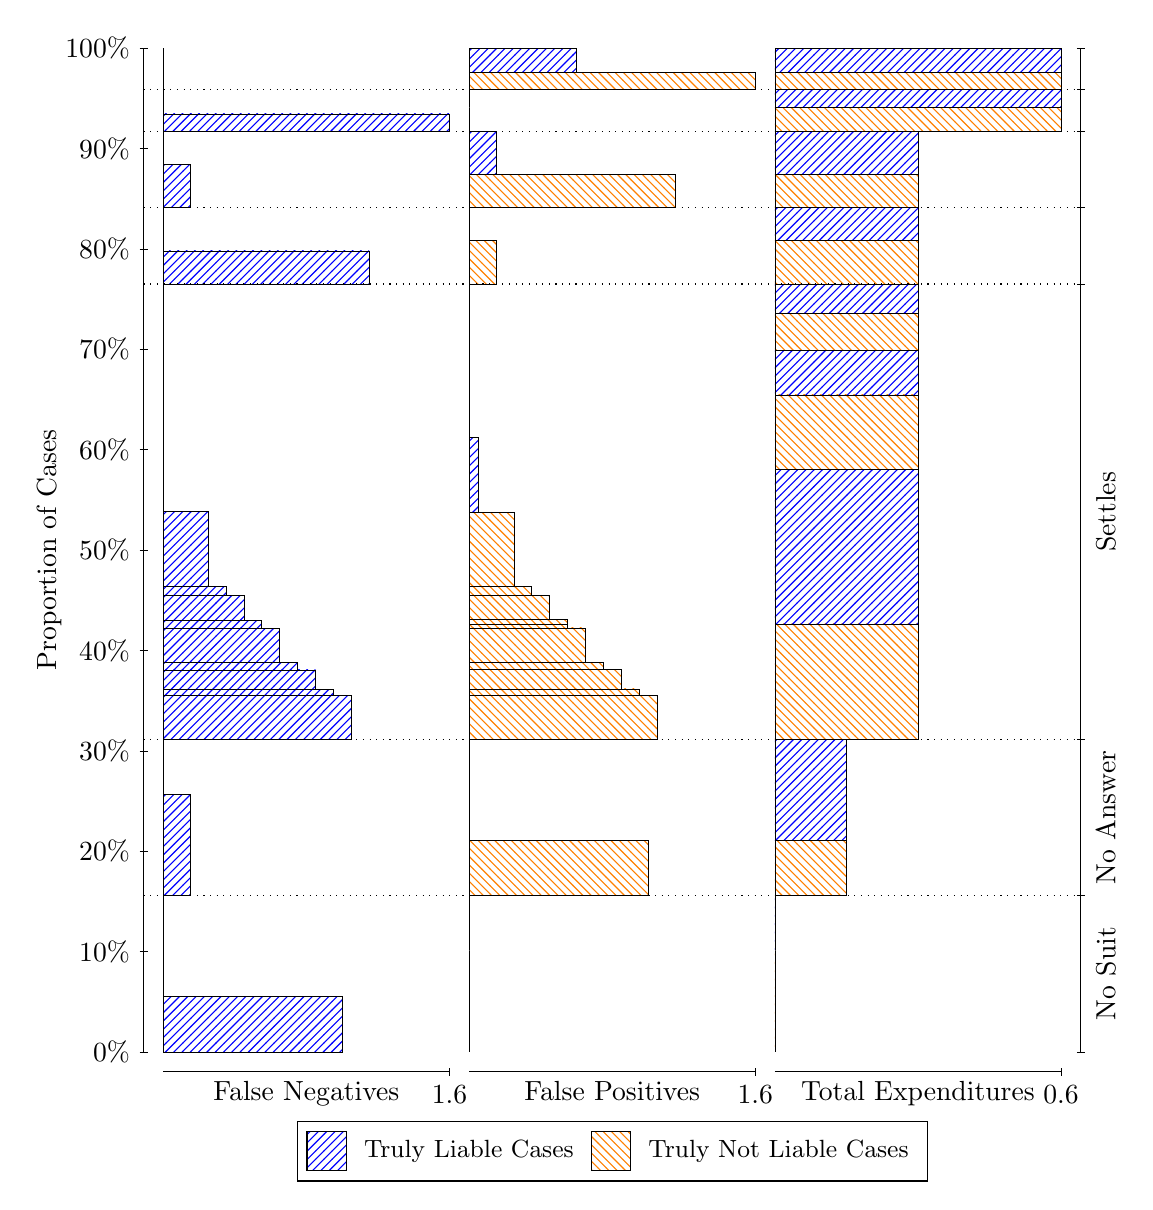
\begin{tikzpicture}
\draw[black, very thin] (1.5,1.75) -- (1.5,14.5);
\node[rotate=90, anchor=center] at (0.3, 8.125) {Proportion of Cases};
\draw[black, very thin] (1.45,1.75) -- (1.55,1.75);
\node[anchor=east] at (1.45, 1.75) {0\%};
\draw[black, very thin] (1.45,3.025) -- (1.55,3.025);
\node[anchor=east] at (1.45, 3.025) {10\%};
\draw[black, very thin] (1.45,4.3) -- (1.55,4.3);
\node[anchor=east] at (1.45, 4.3) {20\%};
\draw[black, very thin] (1.45,5.575) -- (1.55,5.575);
\node[anchor=east] at (1.45, 5.575) {30\%};
\draw[black, very thin] (1.45,6.85) -- (1.55,6.85);
\node[anchor=east] at (1.45, 6.85) {40\%};
\draw[black, very thin] (1.45,8.125) -- (1.55,8.125);
\node[anchor=east] at (1.45, 8.125) {50\%};
\draw[black, very thin] (1.45,9.4) -- (1.55,9.4);
\node[anchor=east] at (1.45, 9.4) {60\%};
\draw[black, very thin] (1.45,10.675) -- (1.55,10.675);
\node[anchor=east] at (1.45, 10.675) {70\%};
\draw[black, very thin] (1.45,11.95) -- (1.55,11.95);
\node[anchor=east] at (1.45, 11.95) {80\%};
\draw[black, very thin] (1.45,13.225) -- (1.55,13.225);
\node[anchor=east] at (1.45, 13.225) {90\%};
\draw[black, very thin] (1.45,14.5) -- (1.55,14.5);
\node[anchor=east] at (1.45, 14.5) {100\%};

\draw[black, very thin] (13.4,1.75) -- (13.4,14.5);
\draw[black, very thin] (13.35,1.75) -- (13.45,1.75);
\node[anchor=west] at (13.35, 1.75) {};
\draw[black, very thin] (13.35,3.7404) -- (13.45,3.7404);
\node[anchor=west] at (13.35, 3.7404) {};
\draw[black, very thin] (13.35,5.7162) -- (13.45,5.7162);
\node[anchor=west] at (13.35, 5.7162) {};
\draw[black, very thin] (13.35,11.503) -- (13.45,11.503);
\node[anchor=west] at (13.35, 11.503) {};
\draw[black, very thin] (13.35,12.48) -- (13.45,12.48);
\node[anchor=west] at (13.35, 12.48) {};
\draw[black, very thin] (13.35,13.44) -- (13.45,13.44);
\node[anchor=west] at (13.35, 13.44) {};
\draw[black, very thin] (13.35,13.97) -- (13.45,13.97);
\node[anchor=west] at (13.35, 13.97) {};
\draw[black, very thin] (13.35,14.5) -- (13.45,14.5);
\node[anchor=west] at (13.35, 14.5) {};

\draw[black, very thin, pattern color=blue, pattern=north east lines] (1.75,1.75) rectangle (4.0208,2.4515);
\draw[black, very thin, pattern color=orange, pattern=north west lines] (1.75,2.4515) rectangle (1.75,3.7404);
\draw[black, very thin, pattern color=blue, pattern=north east lines] (1.75,3.7404) rectangle (2.0906,5.0222);
\draw[black, very thin, pattern color=orange, pattern=north west lines] (1.75,5.0222) rectangle (1.75,5.7162);
\draw[black, very thin, pattern color=blue, pattern=north east lines] (1.75,5.7162) rectangle (4.1344,6.2809);
\draw[black, very thin, pattern color=blue, pattern=north east lines] (1.75,6.2809) rectangle (3.9073,6.3594);
\draw[black, very thin, pattern color=blue, pattern=north east lines] (1.75,6.3594) rectangle (3.6802,6.6025);
\draw[black, very thin, pattern color=blue, pattern=north east lines] (1.75,6.6025) rectangle (3.4531,6.6941);
\draw[black, very thin, pattern color=blue, pattern=north east lines] (1.75,6.6941) rectangle (3.226,7.1289);
\draw[black, very thin, pattern color=blue, pattern=north east lines] (1.75,7.1289) rectangle (2.999,7.2356);
\draw[black, very thin, pattern color=blue, pattern=north east lines] (1.75,7.2356) rectangle (2.7719,7.5445);
\draw[black, very thin, pattern color=blue, pattern=north east lines] (1.75,7.5445) rectangle (2.5448,7.6644);
\draw[black, very thin, pattern color=blue, pattern=north east lines] (1.75,7.6644) rectangle (2.3177,8.6133);
\draw[black, very thin, pattern color=orange, pattern=north west lines] (1.75,8.6133) rectangle (1.75,11.503);
\draw[black, very thin, pattern color=blue, pattern=north east lines] (1.75,11.503) rectangle (4.3615,11.925);
\draw[black, very thin, pattern color=orange, pattern=north west lines] (1.75,11.925) rectangle (1.75,12.48);
\draw[black, very thin, pattern color=blue, pattern=north east lines] (1.75,12.48) rectangle (2.0906,13.022);
\draw[black, very thin, pattern color=orange, pattern=north west lines] (1.75,13.022) rectangle (1.75,13.44);
\draw[black, very thin, pattern color=blue, pattern=north east lines] (1.75,13.44) rectangle (5.3833,13.664);
\draw[black, very thin, pattern color=orange, pattern=north west lines] (1.75,13.664) rectangle (1.75,13.97);
\draw[black, very thin, pattern color=orange, pattern=north west lines] (1.75,13.97) rectangle (1.75,14.194);
\draw[black, very thin, pattern color=blue, pattern=north east lines] (1.75,14.194) rectangle (1.75,14.5);
\draw[black, very thin, pattern color=orange, pattern=north west lines] (5.6333,1.75) rectangle (5.6333,3.039);
\draw[black, very thin, pattern color=blue, pattern=north east lines] (5.6333,3.039) rectangle (5.6333,3.7404);
\draw[black, very thin, pattern color=orange, pattern=north west lines] (5.6333,3.7404) rectangle (7.9042,4.4344);
\draw[black, very thin, pattern color=blue, pattern=north east lines] (5.6333,4.4344) rectangle (5.6333,5.7162);
\draw[black, very thin, pattern color=orange, pattern=north west lines] (5.6333,5.7162) rectangle (8.0177,6.2822);
\draw[black, very thin, pattern color=orange, pattern=north west lines] (5.6333,6.2822) rectangle (7.7906,6.3623);
\draw[black, very thin, pattern color=orange, pattern=north west lines] (5.6333,6.3623) rectangle (7.5635,6.6094);
\draw[black, very thin, pattern color=orange, pattern=north west lines] (5.6333,6.6094) rectangle (7.3365,6.7019);
\draw[black, very thin, pattern color=orange, pattern=north west lines] (5.6333,6.7019) rectangle (7.1094,7.1364);
\draw[black, very thin, pattern color=orange, pattern=north west lines] (5.6333,7.1364) rectangle (6.8823,7.1866);
\draw[black, very thin, pattern color=orange, pattern=north west lines] (5.6333,7.1866) rectangle (6.8823,7.2413);
\draw[black, very thin, pattern color=orange, pattern=north west lines] (5.6333,7.2413) rectangle (6.6552,7.5443);
\draw[black, very thin, pattern color=orange, pattern=north west lines] (5.6333,7.5443) rectangle (6.4281,7.6606);
\draw[black, very thin, pattern color=orange, pattern=north west lines] (5.6333,7.6606) rectangle (6.201,8.6055);
\draw[black, very thin, pattern color=blue, pattern=north east lines] (5.6333,8.6055) rectangle (5.7469,9.5544);
\draw[black, very thin, pattern color=blue, pattern=north east lines] (5.6333,9.5544) rectangle (5.6333,11.503);
\draw[black, very thin, pattern color=orange, pattern=north west lines] (5.6333,11.503) rectangle (5.974,12.057);
\draw[black, very thin, pattern color=blue, pattern=north east lines] (5.6333,12.057) rectangle (5.6333,12.48);
\draw[black, very thin, pattern color=orange, pattern=north west lines] (5.6333,12.48) rectangle (8.2448,12.898);
\draw[black, very thin, pattern color=blue, pattern=north east lines] (5.6333,12.898) rectangle (5.974,13.44);
\draw[black, very thin, pattern color=orange, pattern=north west lines] (5.6333,13.44) rectangle (5.6333,13.746);
\draw[black, very thin, pattern color=blue, pattern=north east lines] (5.6333,13.746) rectangle (5.6333,13.97);
\draw[black, very thin, pattern color=orange, pattern=north west lines] (5.6333,13.97) rectangle (9.2667,14.194);
\draw[black, very thin, pattern color=blue, pattern=north east lines] (5.6333,14.194) rectangle (6.9958,14.5);
\draw[black, very thin, pattern color=orange, pattern=north west lines] (9.5167,1.75) rectangle (9.5167,3.039);
\draw[black, very thin, pattern color=blue, pattern=north east lines] (9.5167,3.039) rectangle (9.5167,3.7404);
\draw[black, very thin, pattern color=orange, pattern=north west lines] (9.5167,3.7404) rectangle (10.425,4.4344);
\draw[black, very thin, pattern color=blue, pattern=north east lines] (9.5167,4.4344) rectangle (10.425,5.7162);
\draw[black, very thin, pattern color=orange, pattern=north west lines] (9.5167,5.7162) rectangle (11.333,7.1866);
\draw[black, very thin, pattern color=blue, pattern=north east lines] (9.5167,7.1866) rectangle (11.333,9.1511);
\draw[black, very thin, pattern color=orange, pattern=north west lines] (9.5167,9.1511) rectangle (11.333,10.096);
\draw[black, very thin, pattern color=blue, pattern=north east lines] (9.5167,10.096) rectangle (11.333,10.661);
\draw[black, very thin, pattern color=orange, pattern=north west lines] (9.5167,10.661) rectangle (11.333,11.135);
\draw[black, very thin, pattern color=blue, pattern=north east lines] (9.5167,11.135) rectangle (11.333,11.503);
\draw[black, very thin, pattern color=orange, pattern=north west lines] (9.5167,11.503) rectangle (11.333,12.057);
\draw[black, very thin, pattern color=blue, pattern=north east lines] (9.5167,12.057) rectangle (11.333,12.48);
\draw[black, very thin, pattern color=orange, pattern=north west lines] (9.5167,12.48) rectangle (11.333,12.898);
\draw[black, very thin, pattern color=blue, pattern=north east lines] (9.5167,12.898) rectangle (11.333,13.44);
\draw[black, very thin, pattern color=orange, pattern=north west lines] (9.5167,13.44) rectangle (13.15,13.746);
\draw[black, very thin, pattern color=blue, pattern=north east lines] (9.5167,13.746) rectangle (13.15,13.97);
\draw[black, very thin, pattern color=orange, pattern=north west lines] (9.5167,13.97) rectangle (13.15,14.194);
\draw[black, very thin, pattern color=blue, pattern=north east lines] (9.5167,14.194) rectangle (13.15,14.5);
\draw[black, dotted] (1.5,3.7404) -- (13.4,3.7404);
\draw[black, dotted] (1.5,5.7162) -- (13.4,5.7162);
\draw[black, dotted] (1.5,11.503) -- (13.4,11.503);
\draw[black, dotted] (1.5,12.48) -- (13.4,12.48);
\draw[black, dotted] (1.5,13.44) -- (13.4,13.44);
\draw[black, dotted] (1.5,13.97) -- (13.4,13.97);
\draw[black, very thin] (1.75,1.5) -- (5.3833,1.5);
\node[anchor=north] at (3.5667, 1.5) {False Negatives};
\draw[black, very thin] (5.3833,1.45) -- (5.3833,1.55);
\node[anchor=north] at (5.3833, 1.45) {1.6};

\draw[black, very thin] (5.6333,1.5) -- (9.2667,1.5);
\node[anchor=north] at (7.45, 1.5) {False Positives};
\draw[black, very thin] (9.2667,1.45) -- (9.2667,1.55);
\node[anchor=north] at (9.2667, 1.45) {1.6};

\draw[black, very thin] (9.5167,1.5) -- (13.15,1.5);
\node[anchor=north] at (11.333, 1.5) {Total Expenditures};
\draw[black, very thin] (13.15,1.45) -- (13.15,1.55);
\node[anchor=north] at (13.15, 1.45) {0.6};

\node[black, centered, rotate=90] at (13.72, 2.7452) {No Suit};
\node[black, centered, rotate=90] at (13.72, 4.7283) {No Answer};
\node[black, centered, rotate=90] at (13.72, 8.6094) {Settles};





\draw (7.449999999999999,1.5) node[draw=none] (baseCoordinate) {};
\begin{scope}[align=center]
        \matrix[scale=0.5, draw=black, below=0.5cm of baseCoordinate, nodes={draw}, column sep=0.1cm]{
            \node[rectangle, draw, minimum width=0.5cm, minimum height=0.5cm, pattern=north east lines, pattern color=blue] {}; &
            \node[draw=none, font=\small] (B) {Truly Liable Cases}; &
            \node[rectangle, draw, minimum width=0.5cm, minimum height=0.5cm, pattern=north west lines, pattern color=orange] {}; &
            \node[draw=none, font=\small] (B) {Truly Not Liable Cases}; \\
            };
\end{scope}

\end{tikzpicture}
\end{document}